\chapter{Разработка мобильного приложения}\label{Bib_chapter}


\section{Структура мобильного приложения Diabetic Diary}

Используя стратегию модульности, на рисунке \ref{fig:AppModul} изображена свзять модульной структуры.

\begin{figure}[h!]
    \begin{center}
        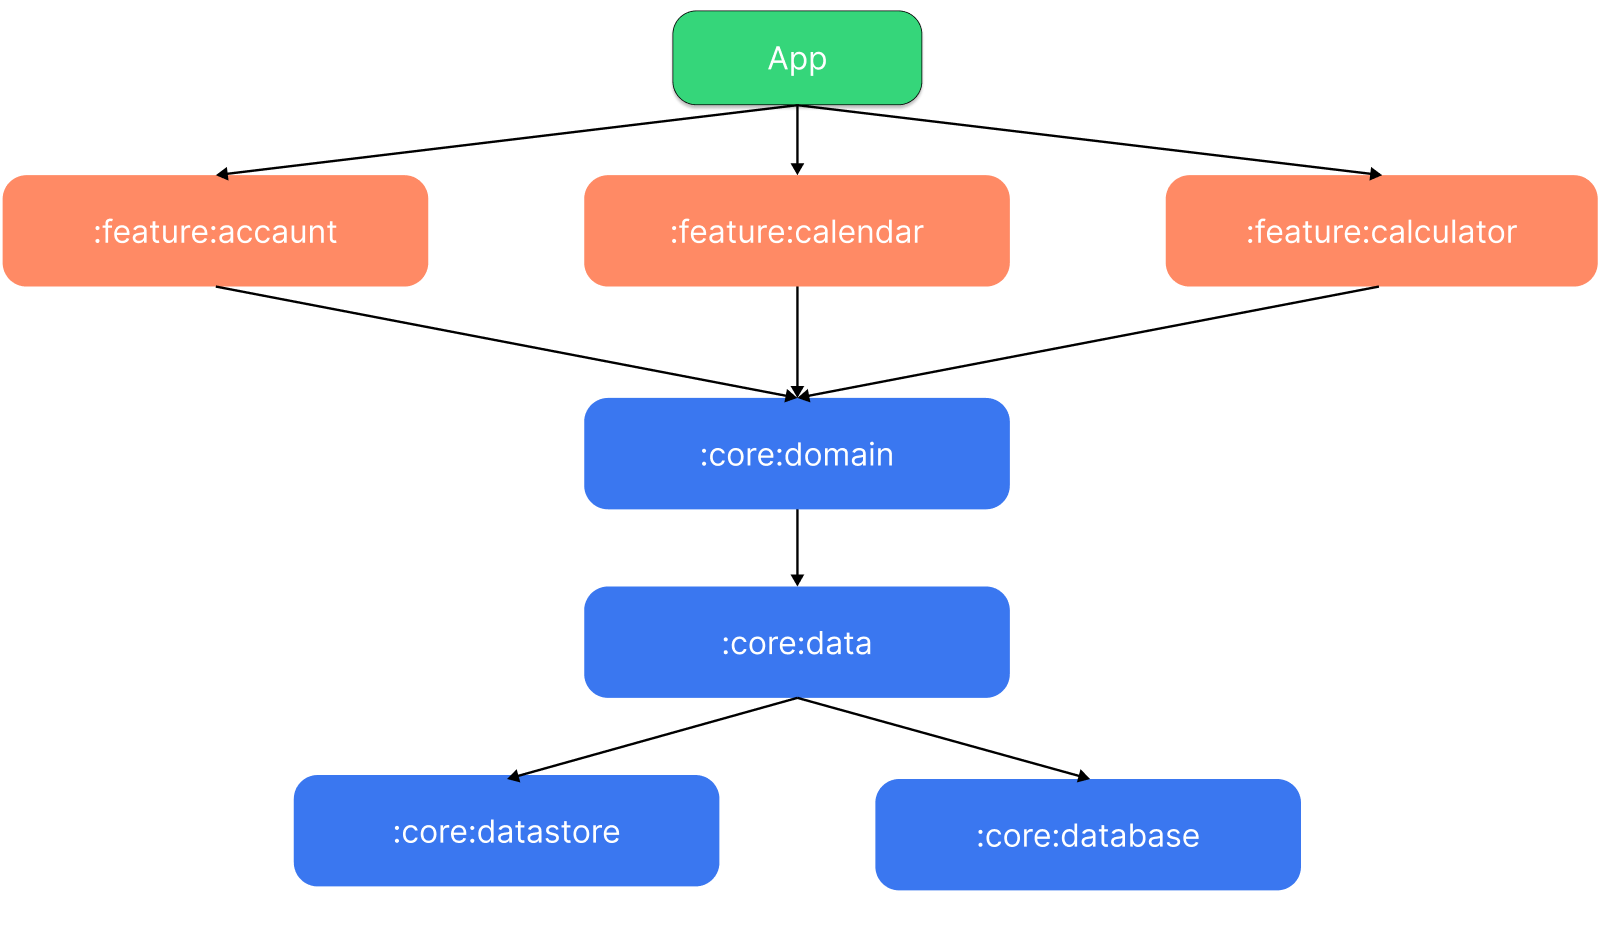
\includegraphics[width=0.8\hsize]{fig/AppModul.png}\\[2mm]
        \caption{Модульная структура приложения}\label{fig:AppModul}
    \end{center}
\end{figure}

Приложение Diabetic Diary содержит следующие модули:
\begin{enumerate}
    \item app. Объединяет все необходимое для правильной работы приложения. Это включает в себя создание пользовательского интерфейса и навигацию;
    \item feature. Содержат компоненты пользовательского интерфейса и ViewModels соответсвующих экранов, которые считывают данные из других модулей;
    \item core:data. Отвечает за извлечение данных приложения из нескольких источников, совместно используемых различными функциями;
    \item core:datastore.  Содержит описание локального хранилища ключ-значений;
    \item core:database. Содержит описание локального хранилища базы данных; 
    \item core:domain. Содержит варианты использования и интерфейсы репозиториев.
\end{enumerate}



На следующей диаграмме показаны события, которые происходят в приложении, и то, как данные поступают из соответствующих объектов, следуя принципам чистой архитектуры (рисунок \ref{fig:AppArch}).

\begin{figure}[h!]
    \begin{center}
        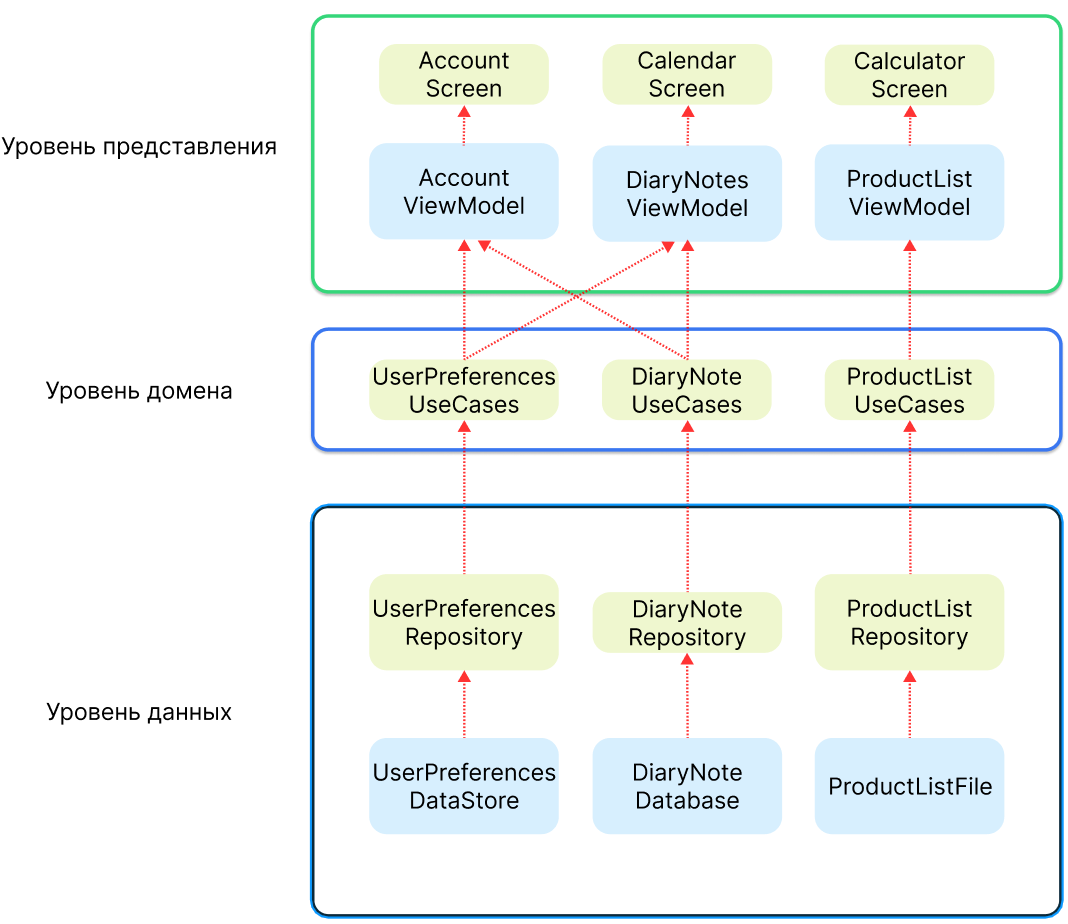
\includegraphics[width=0.9\hsize]{fig/AppArch.png}\\[2mm]
        \caption{Архитектура }\label{fig:AppArch}
    \end{center}
\end{figure}


\section{Работа с внедрением зависимостей Hilt}

Как только Hilt настроен в классе Application и доступен компонент уровня приложения, Hilt может предоставлять зависимости другим классам Android, которые имеют аннотацию \verb|@AndroidEntryPoint|
, в приложении это MainActivity.

Модуль Hilt -- это класс, который аннотируется с помощью \verb|@Module|, он информирует Hilt о том, как предоставлять экземпляры определенных типов.

Аннотация \verb|@Provide| используется для указания метода, который создает и предоставляет зависимость. Этот метод должен быть определен в модуле

Аннотация \verb|@Singleton| используется для указания, что зависимость должна быть создана только один раз и предоставлена всем компонентам, которые требуют этой зависимости, в течение всего жизненного цикла приложения.

Пример 


Чтобы выполнить внедрение класса, Hilt должен знать, как предоставить экземпляры необходимых зависимостей из соответствующего компонента. Одним из способов предоставления информации о привязке к Hilt является использование аннотации \verb|@Inject| в конструкторе класса (листинг \ref{ls:AppB1}).

\begin{lstlisting}[caption={Пример аннотации Inject}, label={ls:AppB1}]
@HiltViewModel
class DiaryNotesViewModel @Inject constructor(
    private val diaryNoteUseCases: DiaryNoteUseCases,
    savedStateHandle: SavedStateHandle
) : ViewModel(){…}
\end{lstlisting}




\section{Работа с локальными данными приложения}

\subsection{Хранение данных с помощью Room}
\subsection{Хранение данных с помощью DataStore}
\subsection{Хранение данных с помощью файловой системы}

\section{Разработка пользовательского интерфейса с Compose}



